\chapter{Cosmic rays}
\label{ch:cosmic-rays}


\section{History of cosmic-ray research}

Cosmic rays were `discovered' in 1835, i.e.\ their effects were detected. An electroscope was seen to discharge at unexpected rates.

The effects of low-energy solar cosmic rays were seen much earlier, namely in the form of the aurora borealis and aurora australis (named such in the 17th century, but many ancient folk tales about this phenomena exist). An example of the aurora can be seen in \cref{fig:aurora}. The aurora is caused by disturbances in Earths' magnetosphere, often due to solar winds, which cause charged particles to follow the magnetic field lines into the atmosphere where they will excite and ionize oxygen and nitrogen atoms. When these deexcite or recombine the observed colors are produced.

The cause of the effect detected in the electroscope was long thought to be of other origins. In .. the discovery of X-rays presented a good candidate, and the existence of  spotaneous radioactivity solidified this as the likely cause being a terrestial source. The term cosmic ray implies that these are photons. However, experiments showed a dependence on latitude for the flux of the cosmic rays, which indicate that these rays had a charge, as ... terra model.. showed that the magnetic field of Earth deflected these particles to the poles. Experiments that took to the sky showed that higher densities of these ionizations were to be found at high altitudes. The discovery of extensive air showers (EAS) by Auger and Rossi simultaneously/independently ignited the cosmic-ray research field. New possibilities for studing cosmic rays were found.

\begin{figure}
    \centering
    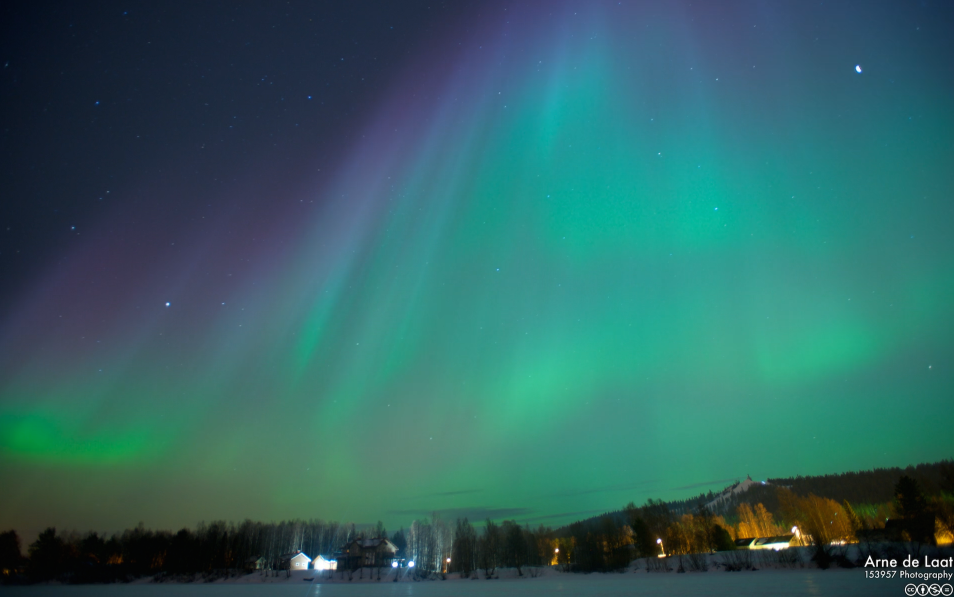
\includegraphics[width=0.6\textwidth]{plots/cosmic-rays/aurora.png}
    \caption{The aurora borealis as seen in Rovanemi, Finland on 17 March 2015, St. Patricks day. The large aurora activity on that day was due to a G4 geomagnetic storm on the sun on the 15th.}
    \label{fig:aurora}
\end{figure}


\subsection{Balloon experiments}

Other experiments also took to the sky because that is where the cosmic rays could be detected before they underwent collisions with particles in the atmosphere. Ground based experiments only see the remnants of the EAS. Being able to directly detect the particle has many advantages. Such as better energy and direction resolution, and easier identification of the particle. The main downside is the flux of cosmic rays decreases steeply when looking at higher energy cosmic rays. Ideally you would have a large detector surface with a very long exposure time. Unfortunately a detector that has be flown at the top of the atmosphere or in space can only be so big before it costs to much. And balloon experiments are short runs where the balloon only stays up ... days/months? So the high-energy limit for these experiments is limited by their size and operational length.

- List evolution of balloon experiments.
- List major contributions by some experiments.

There have been many such experiments, all together providing a very detailed picture of the low energy cosmic-ray spectrum. The per-nucleus spectrum of such experiments is shown in \cref{fig:low_e_spectrum}.

\begin{figure}
    \centering
    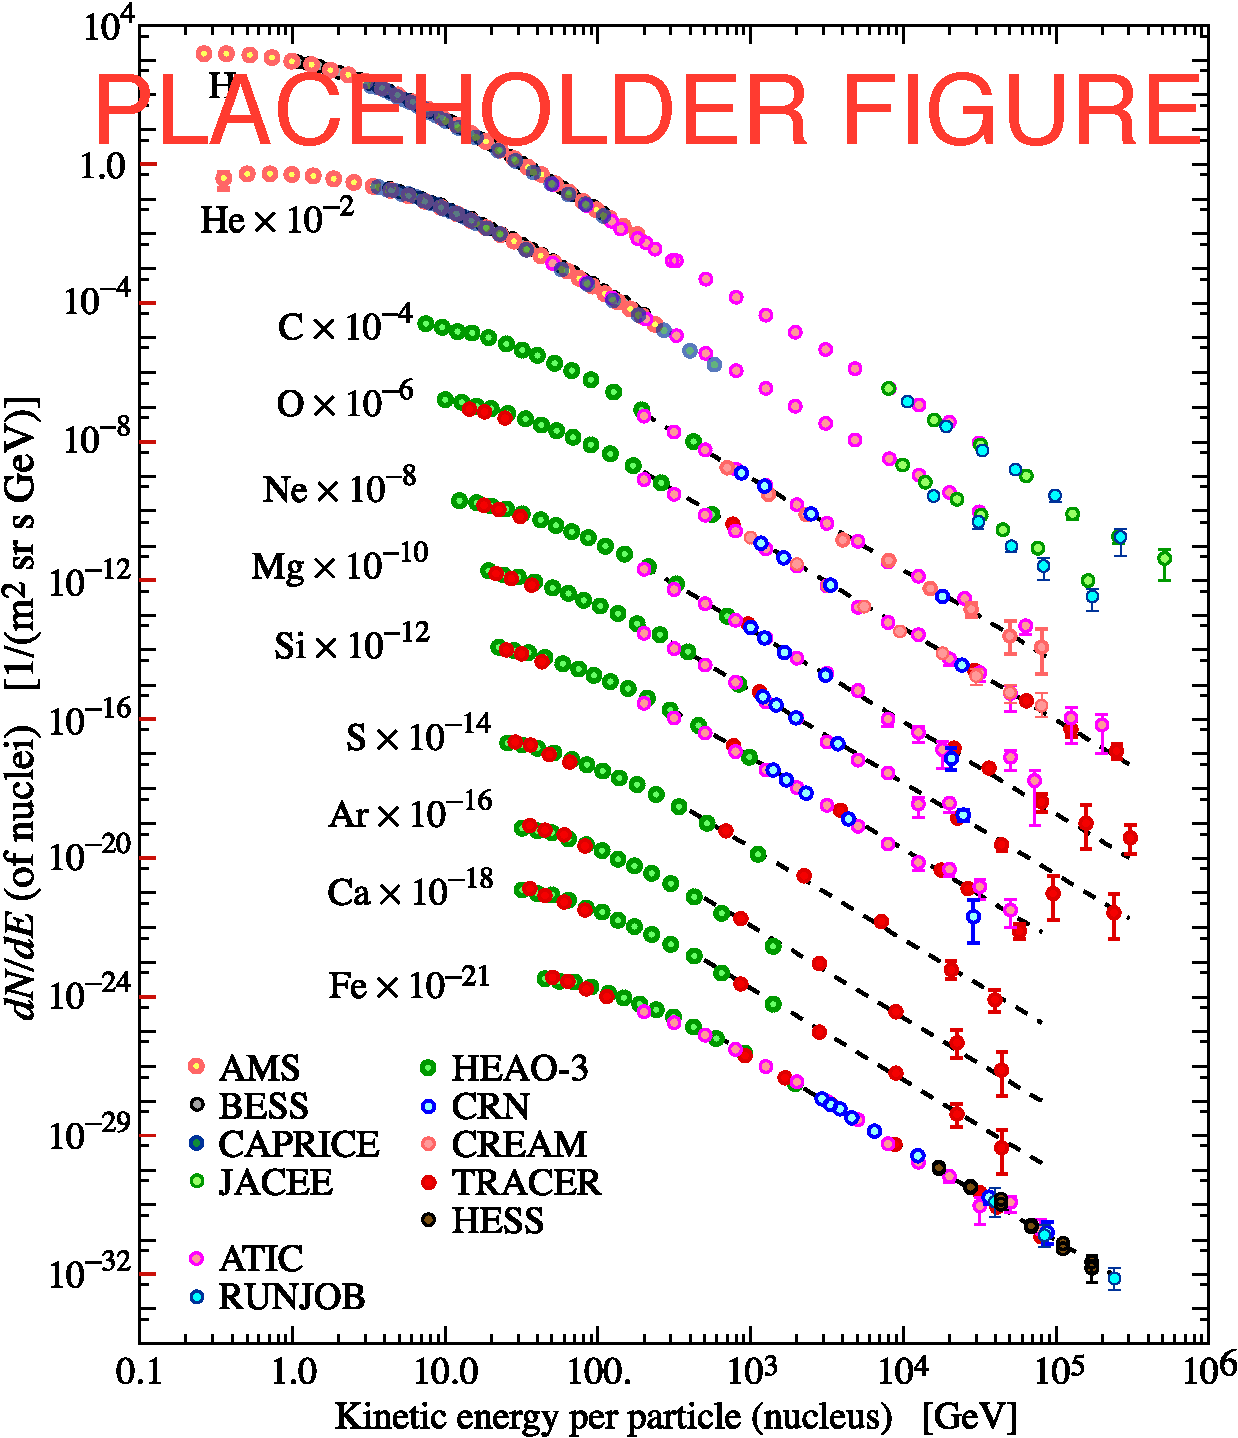
\includegraphics[width=0.6\textwidth]
                    {plots/cosmic-rays/PDG_28_1_fluxes_per_nucleus}
    \caption{Per nucleus spectrum of cosmic-rays from the PDG.}
    \label{fig:low_e_spectrum}
\end{figure}


\subsection{Ground-based experiments}

As explained in the previous section direct measurements of high energetic (>.. eV) is difficult, but the nature of the EAS means that other their showers are detectable over large distances on the ground. It is cheaper to operate such an experiment over a large period of time. Different experiments have focused on different aspects of air showers. Some looking for the highest energies, others for filling in the intermediate range. Some try to sample the shower front as accurately as possible. Some experiments look at the shower development in the atmosphere by looking at the fluorescence created by the shower. In recent years radio detection of air showers has been developed. These look for a signature signal created in radio, caused by the magneticfield moving the electrons and positrons in opposite directions.

Some detector arrays are situated high up, closer to Xmax, this has the advantage that less extinction and scattering has occured in the EAS. After Xmax particle extinction becomes dominated, versus new particle creation. 

This also means that the particle density for lower energy showers is higher, however, using coincidence triggering with detectors sufficiently spaced these should be easily separated from the desired signals.

Notable ground-based experiments are ....

AGASA, KASCADE-Grande, Auger Observatory, TA, Tibet, Fly's Eye, Havanah Park, Volcano Ranch, HiRes, IceTop, CASA-MIA, Tien-Shan, Ahemo, MGU, Grigorov

Rossi/Zatsepin and other early experiments..


\begin{figure}
    \centering
    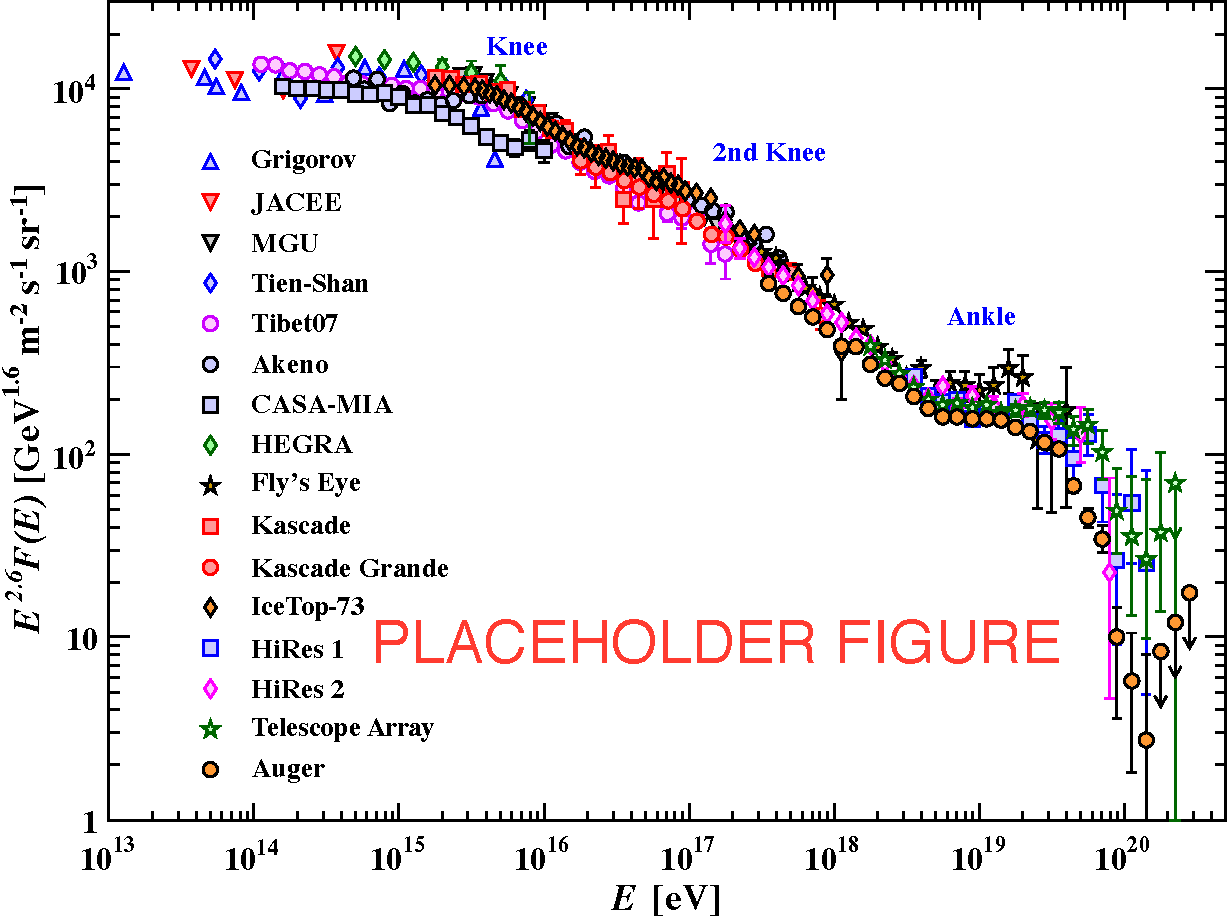
\includegraphics[width=0.6\textwidth]
                    {plots/cosmic-rays/PDG_28_8_all_particle_spectrum}
    \caption{The all particle spectrum of cosmic-rays from the PDG.}
    \label{fig:spectrum}
\end{figure}



\section{Air-shower physics}

Main proccess, production channels. hadronic, electromagnetic, muons..


\section{Air-shower simulations}

Collider contributions to cross sections.

LHC approaches interesting energy range, unfortunately only p-p, Pb-p, and Pb-Pb. For cosmic rays the interessting collisions would be p-O, p-N, and p-C. Because these are more common elements in the atmosphere and likely part of the first interaction. Also the forward region (low/high rapidity region, low pt) in these collisions are the interessting reagions for cosmic ray physics. Unfortunately the design of these colliders does not allow for detectors close to the beam and close to the collision.


\section{\hisparc for outreach and research}

The \textbf{Hi}gh \textbf{S}chool \textbf{P}roject on \textbf{A}strophysics \textbf{R}esearch and \textbf{C}osmics (\hisparc) is a ground-based detector experiment. It is not soley intended as an advanced cosmic-ray research experiment, but also as an outreach project which engadges high-school students. Most of the \hisparc detector stations are situated at high schools, and have been built by groups of students from those schools. The building of the detectors takes several days and if done by groups of upto eight students. Because some specialized equipment is required for the construction and to properly supervise the process this is performed at a participating university. On the first day they are intruduced to cosmic-ray physics and assemble the scintillator and lightguide parts of the detector which involves glueing. This glue needs to dry for several days after which the students come again to wrap the detector to make it light tight, as can be seen in \cref{fig:detector-bouw}. Finally the photo multiplier is attached and the detector is tested in the lab before it is placed on the school roof. Students taking physics classes are also encouraged to do their research project on \hisparc. In Dutch this project is called `profielwerkstuk' which is a mandetory part of their final year in high school. This project should be related to a subject in the profile of subjects which they have chosen. In order to assist these students and others that want to work with on cosmic-ray research all data recorded by \hisparc is freely available (licensed under Creative Commons BY-SA 4.0) for use. Moreover, tools are provided to assist in data analysis. On several occasions a symposium was held in which students could present their profielwerkstuk and win a trip to Cern, the subject of their project had to be about a physics field relevant for cosmic rays.

\begin{figure}
    \centering
    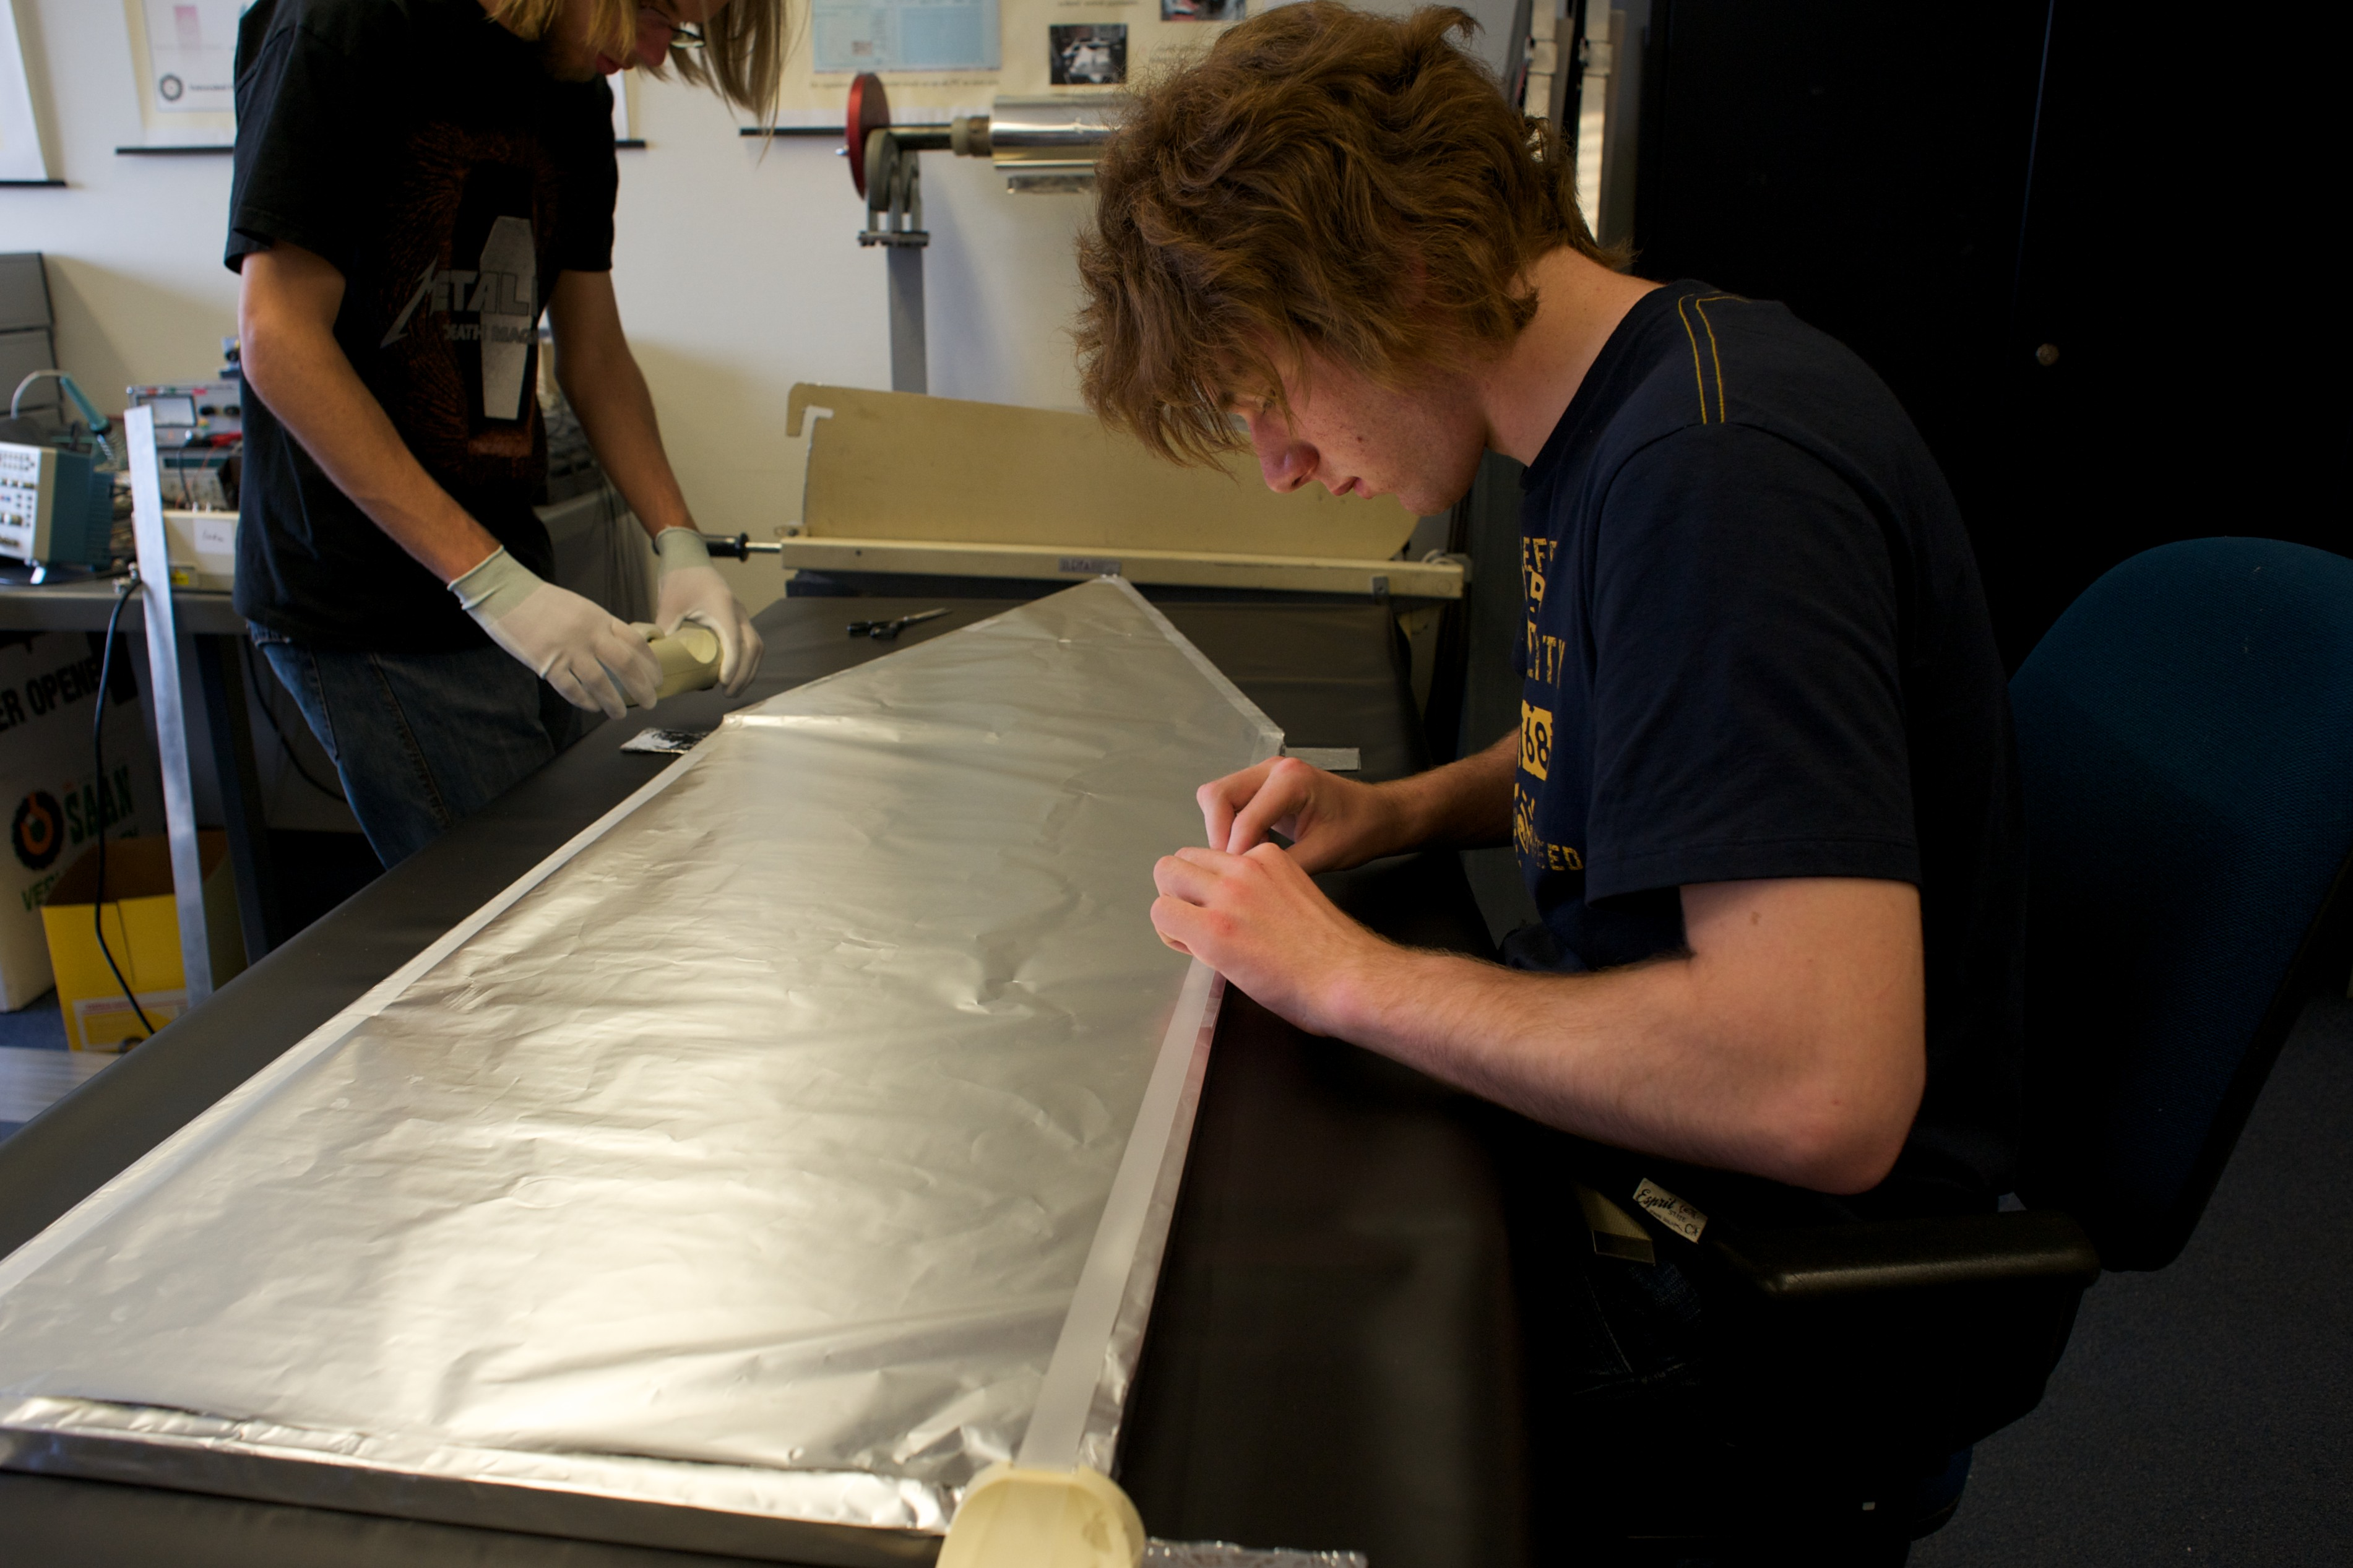
\includegraphics[width=0.6\textwidth]
                    {plots/cosmic-rays/ADL_100352}
    \caption{High-school students work on finishing a detector.}
    \label{fig:detector-bouw}
\end{figure}


\section{The work presented in this thesis}

The goal of the research presented in this thesis is the reconstruction of EAS detected with multiple detector stations from the \hisparc network. For reconstructions an understanding of the individual detectors and detector stations is required. Experiments and simulations have been performed to determine the accuracy and response of the various components.


\subsection{The \hisparc experiment
            (\crefrange{ch:hisparc-experiment}{ch:cluster})}

In the next chapter the overall project is described, including summaries of layered structured of \hisparc is explained. First at the overall project is described. The start and growth of the project are discussed and the organization structure explained.

Then the design an performance of the different scales is discussed. This starts with the individual detectors, the scintillators which detect the passing EAS particles. The construction of the detector has to be practicle enough to be performed by high-school students. There are many interesting aspects concerning the signal strength and timing response of the detectors which is discussed in this part. As explained before/above a single detector is not enough to identify EAS, so multiple detectors are combined to create a detector station which can pick out EAS from the background signals. The readout, trigger logic, and timing of detector stations is explained. A single detector station is small enough to fit on a roof. Multiple detector stations are deployed in the \hisparc project. To combine the data accurate absolute timing is 


\subsection{Software infrastructure
            (\cref{ch:software,ch:data_processing})}



\subsection{Data analysis
            (\cref{ch:simulations,ch:analysis})}



\subsection{Science Park data analysis
            (\cref{ch:network})}



\subsection{Coordinate systems and outreach 
            (\cref{ch:coordinates,ch:outreach})}


















